\documentclass[notes,11pt]{beamer}
%\setbeamertemplate{navigationsymbols}{}
%\colorlet{structure}{blue!50!gray}
\mode<article> % only for the article version
    {
  \usepackage{beamerbasearticle}
  \usepackage{fullpage}
  \usepackage{hyperref}
  \usepackage{multidmedia}
  \usepackage{graphics}
  \usepackage{epsfig}
  \usepackage{graphicx}
   }
\usefonttheme{serif}
\beamertemplateshadingbackground{white!100}{yellow!0}
%\setbeamercolor{title}{fg=red!80!black}
\usepackage{beamerthemeshadow}

\usepackage{pgf,pgfarrows,pgfnodes,pgfautomata,pgfheaps,pgfshade}
\usepackage{amsmath,amscd,amssymb}
\usepackage[latin1]{inputenc}
\usepackage{colortbl}
\usepackage{placeins}


\usepackage{multirow}
\usepackage[english]{babel}
\usepackage{graphics}
\usepackage{epsfig}
\usepackage{graphicx}
%\usefonttheme{serif}
\beamertemplatetransparentcovereddynamic
\newcommand{\mblock}[4]{\ensuremath{\left(\begin{array}{cc}#1&#2\\#3&#4\end{arra
y}\right)}}\newcommand{\vblock}[2]{\ensuremath{\left(\begin{array}{c}\!\!\!#1\\\
!\!\!#2\end{array}\!\!\!\right)}}
\newcommand{\selectpos}[1]{%
   \pgfsetlinewidth{0.6pt}%
   \color{structure}%
   \pgfsetendarrow{\pgfarrowto}%
   \pgfnodeconncurve{machine}{n#1}{90}{-90}{.5cm}{.5cm}%
}
\newtheorem{proposition}{Proposition}%[section]
\newtheorem{remark}{Remark}%[section]
%\newtheorem{lemma}{Lemma}
%\newtheorem{definition}{Definition}
\newcommand{\Lang}[1]{\operatorname{\text{\textsc{#1}}}}
\newcommand{\cells}{\mathcal K}
\newcommand{\edges}{\mathcal S}
\newcommand{\edgesint}{\mathcal S^{int}}
\newcommand{\edgesbound}{\mathcal S^{\partial}}
\newcommand{\eps}{\varepsilon}

\newcommand{\Class}[1]{\operatorname{\mathchoice
  {\text{\normalfont\small #1}}
  {\text{\normalfont\small #1}}
  {\text{\normalfont#1}}
  {\text{\normalfont#1}}}}
\newcommand{\norm}[2]{\ensuremath{\| #1 \|_{#2}}}
\newcommand{\DOF}{\Class{DOF}}
\newcommand{\NOF}{\Class{NOF}}
\newcommand{\DOFpoly}{\Class{DOF}_{\operatorname{poly}}}
\newcommand{\NOFpoly}{\Class{NOF}_{\operatorname{poly}}}
\newcommand{\bb}[1]{\ensuremath{\mathbb{#1}}}%\mathbb works with amsfonts
\newcommand{\seq}[1]{\ensuremath{\left\{ #1 \right\}}}
\newcommand{\ipt}[2]{\ensuremath{\left\langle#1,#2\right\rangle}}
\newcommand{\abs}[1]{\ensuremath{\mid\!\! #1\! \!\mid}}
\newtheorem{theoreme1}{Th\'eor\`eme 1}
 \newtheorem{theoreme2}{Th\'eor\`eme 2}
 \newtheorem{theoreme3}{Th\'eor\`eme3}
 \newtheorem{theoreme4}{Th\'eor\`eme4}
 \newtheorem{theoreme5}{Th\'eor\`eme 5}
 \newtheorem{theoreme6}{ Th\'eor\`eme6}
 \newtheorem{Corollaire}{Corollaire}
 \newtheorem{proposition1}{Proposition}
 \newtheorem{Lemme1}{Lemme1}
\newtheorem{fin}{}
 \newtheorem{Lemme2}{Lemme2}
\newtheorem{proof1}{id\'ee de la preuve}
\newtheorem{proof2}{id\'ee de la preuve}
\newcommand{\Nat}{\mathbb{N}}
\newcommand{\Set}[1]{\{#1\}}
\renewcommand{\div}{\operatorname{div}}
\def \R{\bb{R}}
\def\colorize<#1>{\temporal<#1>{\color{black!30}}% gris avant
{\color{red}}% rouge
{\color{black}}}% noir apr�s

\def\N{\mathbb{N}}
\def\cu {\mbox{\bf curl }}
\def\D{{\mathscr D}}
\def\gr {\mbox{\bf grad }}
\def\c {\mbox{\bf curl }}
\def\phiv{\boldsymbol{\varphi}}
\def\d {\mbox{\rm div }}
\def\R{\mathbb{R}}
\def\dd{\textup{d}}
\def\u{{\textbf {\textit u}}}
\def\vv{{\textbf {\textit v}}}
\def\f{{\textbf {\textit f}}}
\def\g{{\textbf {\textit g}}}
\def\w{{\textbf {\textit w}}}
\def\l{{\boldsymbol {\ell}}}
\def\n{{\textbf {\textit n}}}
\def\h{{\textbf {\textit h}}}
\def\L{{\textbf {\textit L}}}
\def\x{{\textbf {\textit x}}}
\def\z{{\textbf {\textit z}}}
\def\y{{\textbf {\textit y}}}
\def\h{{\textbf {\textit h}}}
\def\F{{\bf F}}
\def\varphiv{\boldsymbol{\varphi}}
\def\psiv{\boldsymbol{\psi}}
\def\gammav{\boldsymbol{\gamma}}
\def\muv{\boldsymbol{\mu}}
\def\etav{\boldsymbol{\eta}}
\def\DD{\mathcal D}
\def\fin {\hbox{\vrule height 5pt width 5pt depth 0pt}}











%\setbeamertemplate{navigationsymbols}{}
%\colorlet{structure}{blue!50!gray}
\mode<article> % only for the article version
    {
  \usepackage{beamerbasearticle}
  \usepackage{fullpage}
  \usepackage{hyperref}
  \usepackage{multidmedia}
  \usepackage{graphics}
  \usepackage{epsfig}
  \usepackage{graphicx}
   }
\usefonttheme{serif}
\beamertemplateshadingbackground{white!100}{yellow!0}
%\setbeamercolor{title}{fg=red!80!black}
\usepackage{beamerthemeshadow}

\usepackage{pgf,pgfarrows,pgfnodes,pgfautomata,pgfheaps,pgfshade}
\usepackage{amsmath,amscd,amssymb}
\usepackage[latin1]{inputenc}
\usepackage{colortbl}
\usepackage{placeins}
\usepackage{multirow}
\usepackage[english]{babel}
\usepackage{graphics}
\usepackage{epsfig}
\usepackage{graphicx}
%\usefonttheme{serif}
\beamertemplatetransparentcovereddynamic



\title [DDSAnalytics]{ATTRITION ANALYSIS}


\author[H. H. NGUYEN] 
{{\sc{Huy Hoang Nguyen}}\\[5pt]
DDS Analytics
 }
 \date {}
\institute[SMU] 

\begin{document}



\frame{

\titlepage
}




\begin{frame}
${}$\\
\begin{center}
\textbf{\color{blue}\Large{Objective}}
\end{center}\medskip

\begin{itemize}
\item<1-> Exploratory Data Analysis  to understand main factors  for Attrition problem
\item<2-> Job Role Trends
\item<3-> Build Models to predict  Salary and Attrition 
\item<4-> Validation of Models for Salary and Attrition 
\item<5-> Create a ShinyApp for data visualization

\end{itemize}

\end{frame}
%%%%%%%

\begin{frame}
\textbf{\color{blue}\large{About me:}} 
\begin{itemize}
\item<1-> Data Cruncher
\item<1-> Hype Crew
\end{itemize}
\end{frame}


%%%%%%%

\begin{frame}
\begin{center}
\textbf{\color{blue}\Large{Exploratory Data Analysis}}
\end{center}\medskip

\begin{figure}
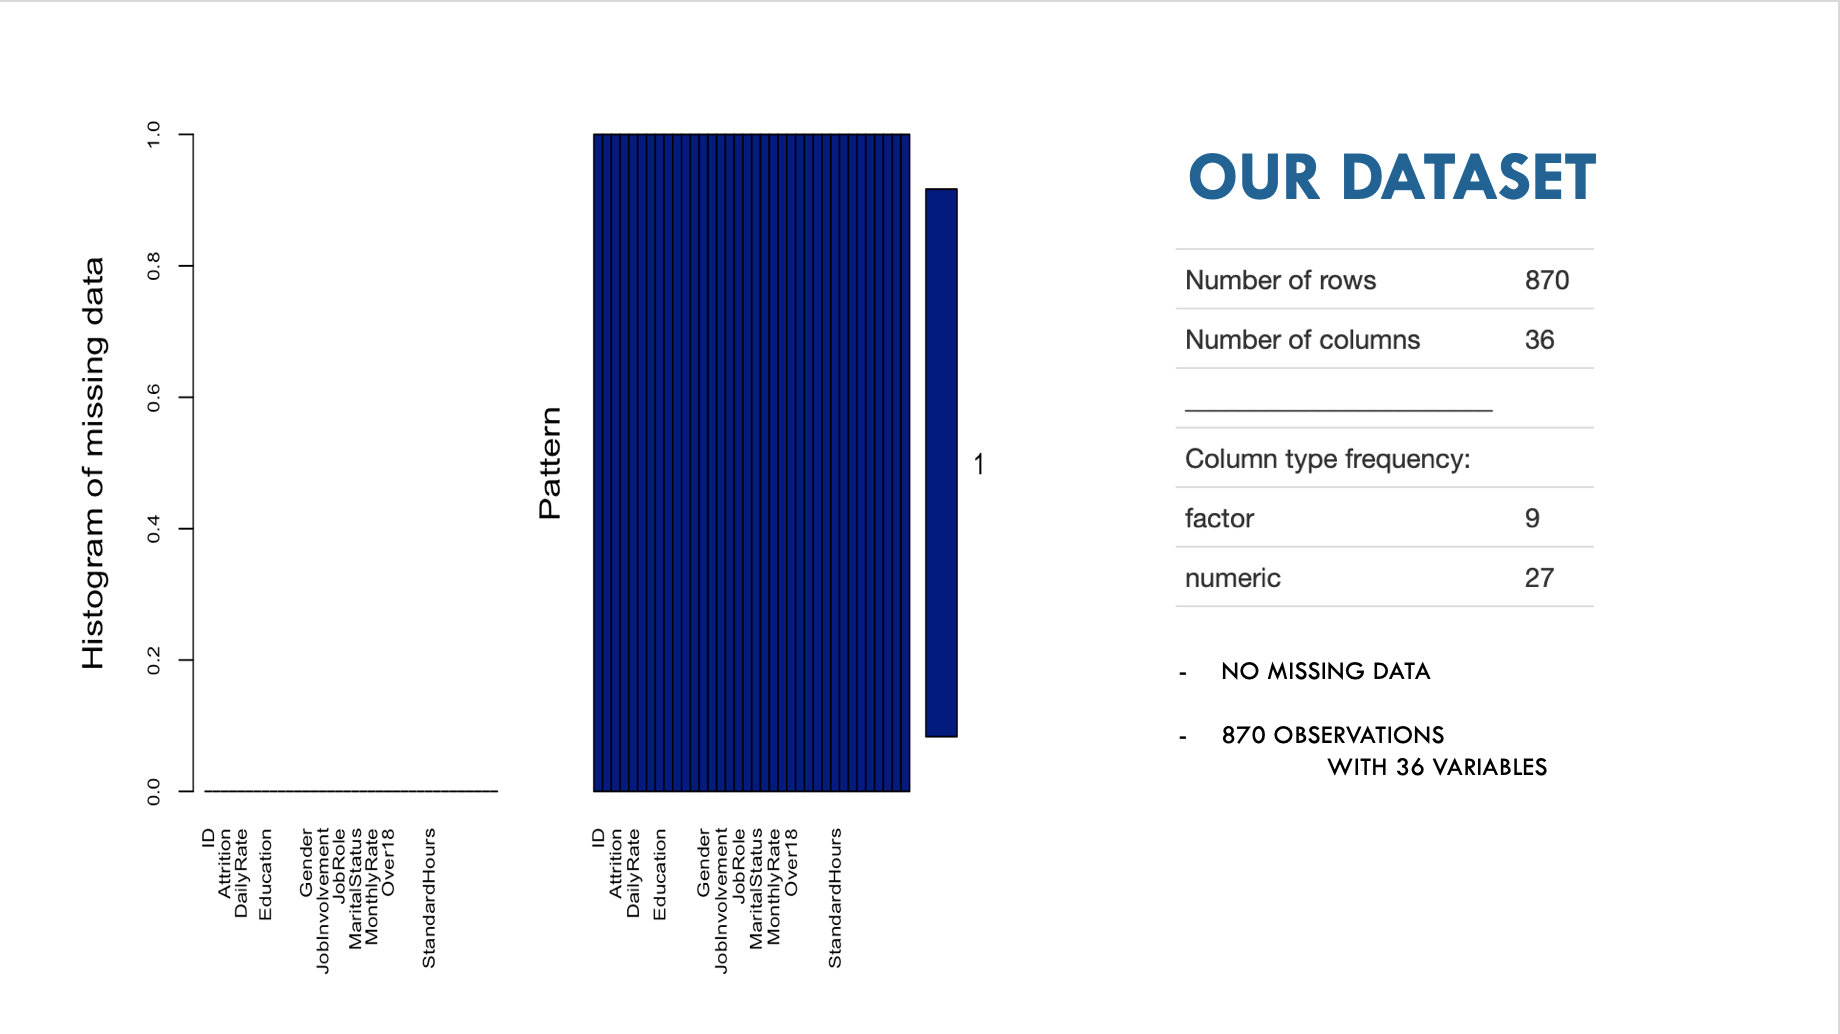
\includegraphics[scale=0.4]{PIC1}
\end{figure}

\end{frame}



%%%%%%%%%
\begin{frame}
\begin{center}
\textbf{\color{blue}\Large{ Attrition}}
\end{center}\medskip
\begin{figure}
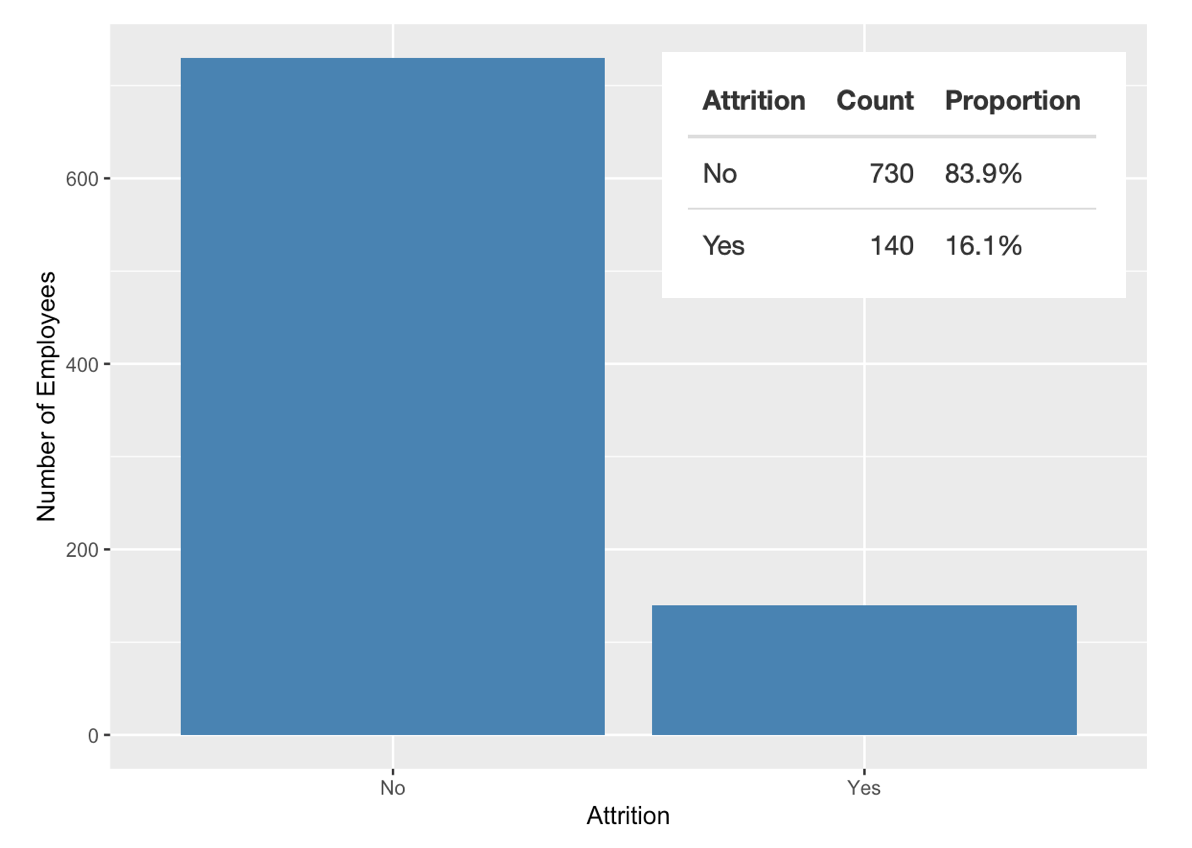
\includegraphics[scale=0.5]{PIC2}
\end{figure}


\end{frame}
%%%%%%%%%






%%%%%%%%%
\begin{frame}
\begin{center}
\textbf{\color{blue}\Large{Monthly Income}}
\end{center}\medskip
\begin{figure}
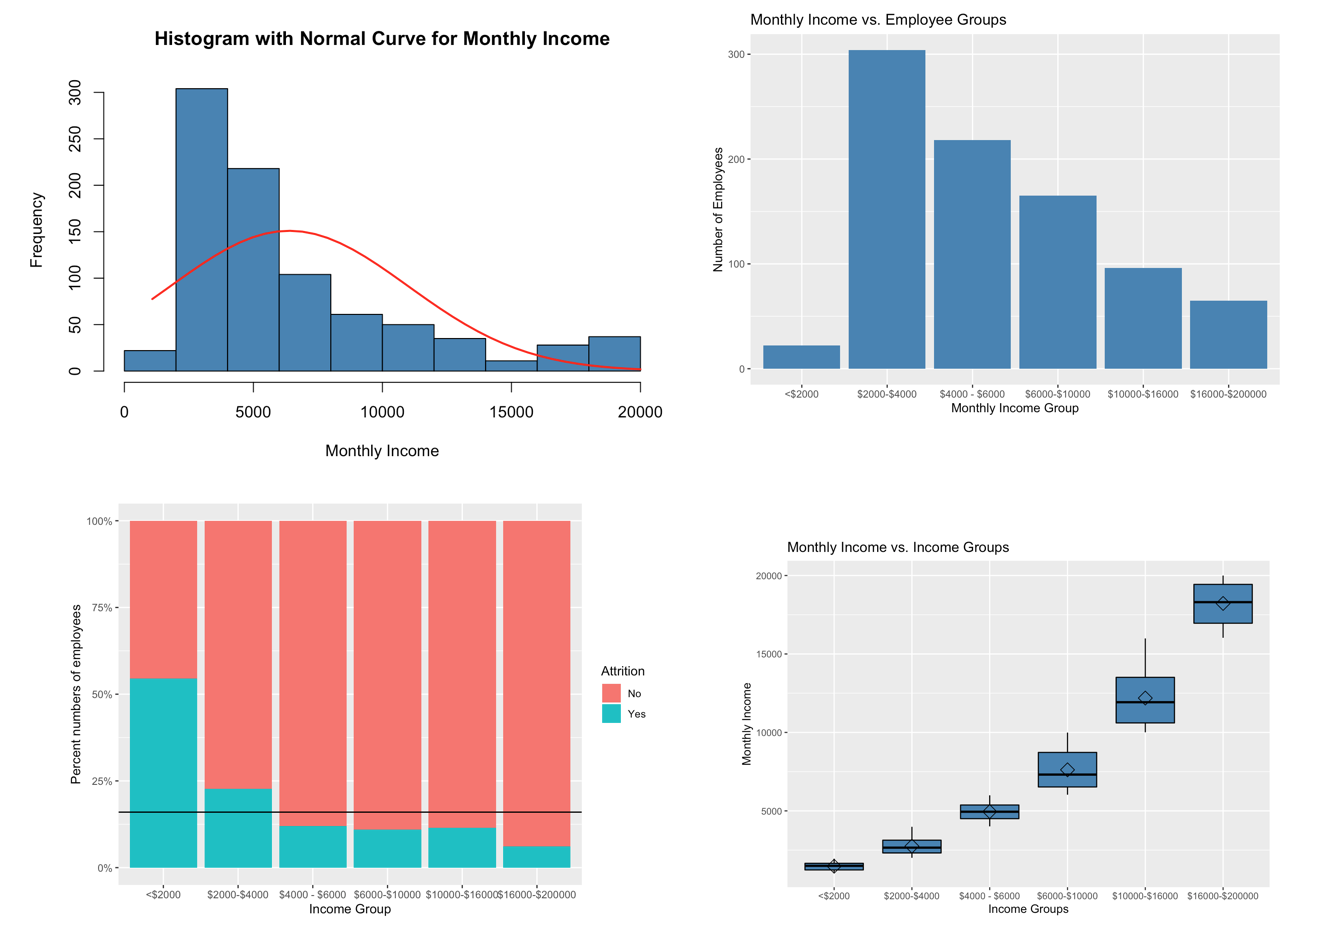
\includegraphics[scale=0.45]{PIC3}
\end{figure}


\end{frame}
%%%%%%%%%


%%%%%%%%%
\begin{frame}
\begin{center}
\textbf{\color{blue}\Large{Job Role vs. Attrition rate}}
\end{center}\medskip
\begin{figure}
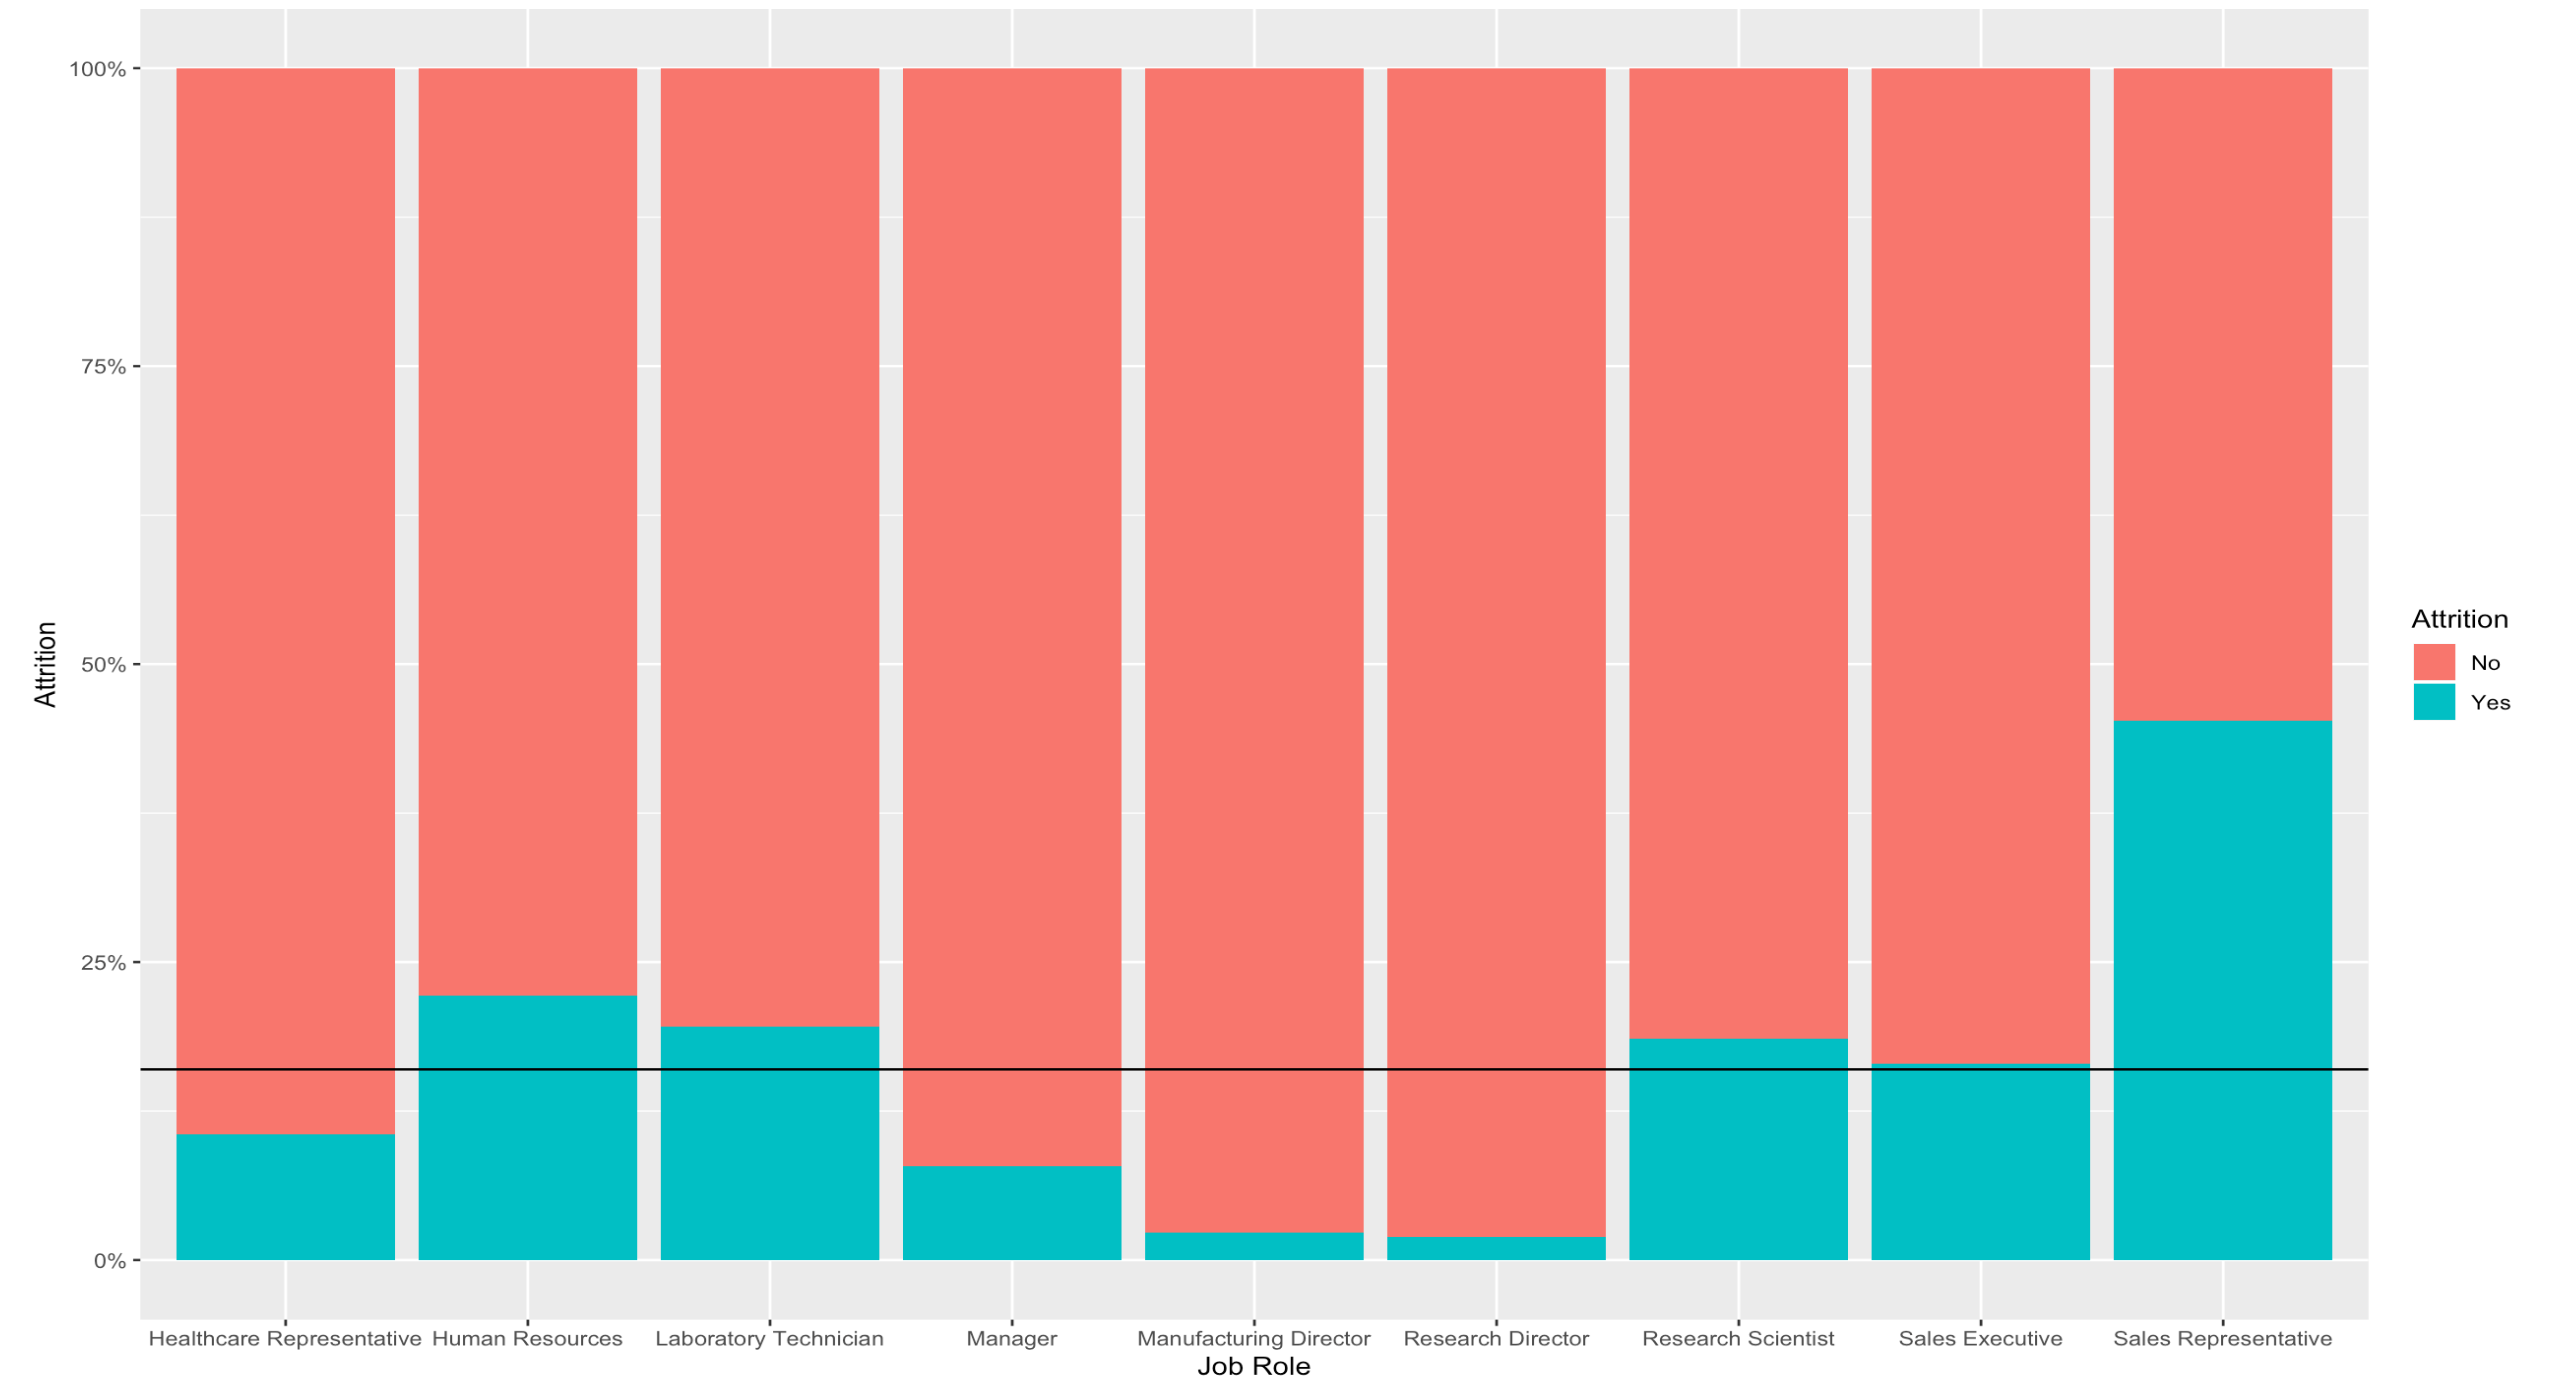
\includegraphics[scale=0.25]{PIC4}
\end{figure}


\end{frame}

%%%%%%%%%%

%%%%%%%%%
\begin{frame}
\begin{center}
\textbf{\color{blue}\Large{Hourly Rate vs Daily Rate vs Monthly Rate vs Monthly Income}}
\end{center}\medskip
\begin{figure}
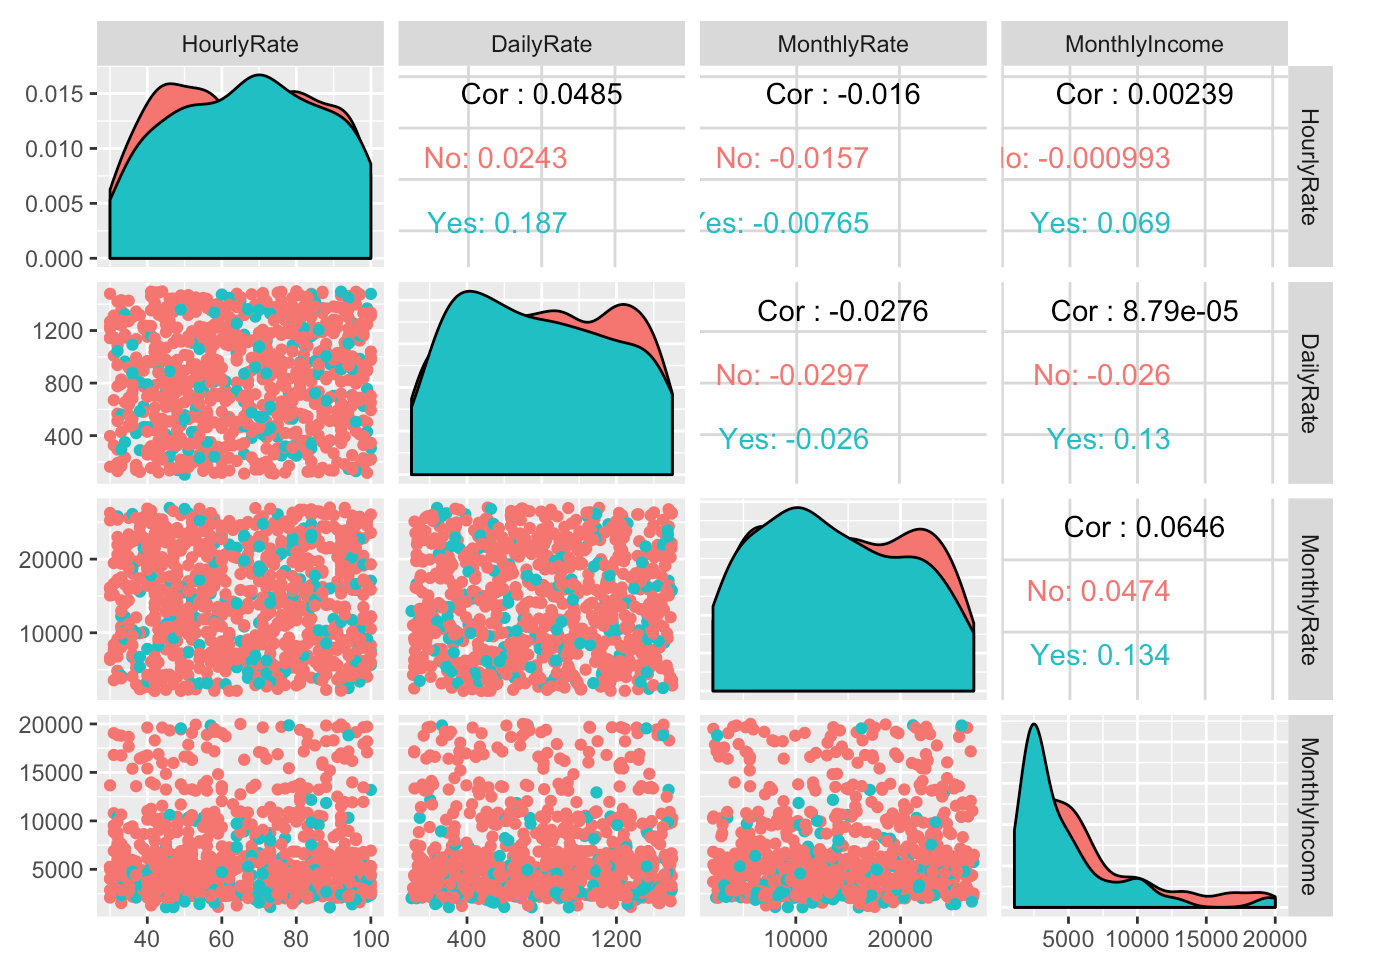
\includegraphics[scale=0.40]{PIC6}
\end{figure}


\end{frame}


%%%%%%%%

\begin{frame}

\begin{figure}
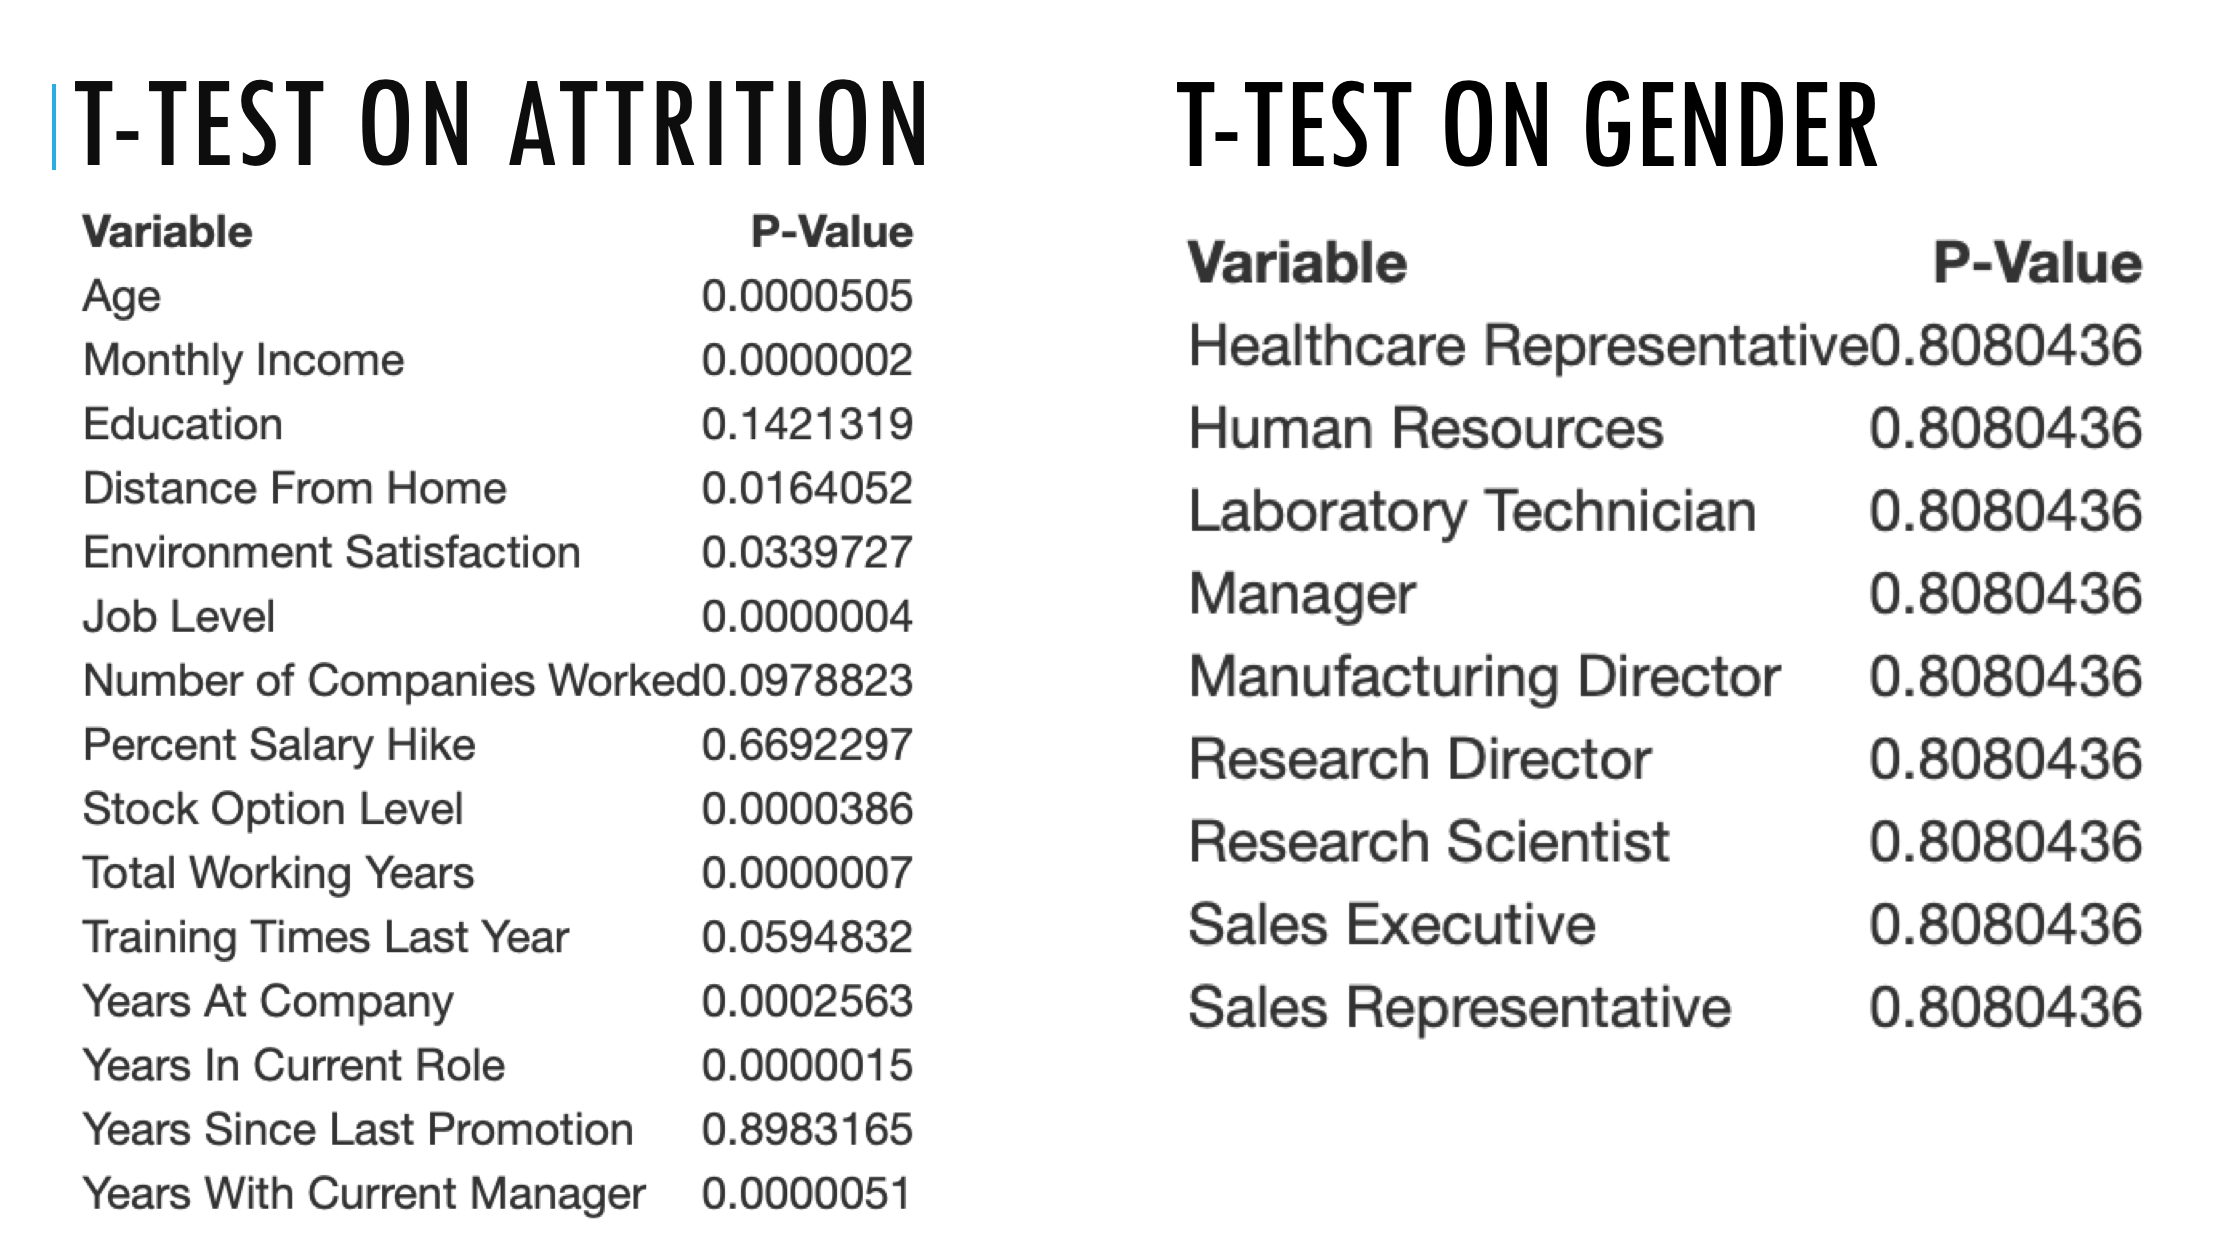
\includegraphics[scale=0.25]{PIC7}
\end{figure}


\end{frame}


%%%%%

%%%%%%%%%
\begin{frame}
\begin{center}
\textbf{\color{blue}\Large{Numeric variables correlation}}
\end{center}\medskip
\begin{figure}
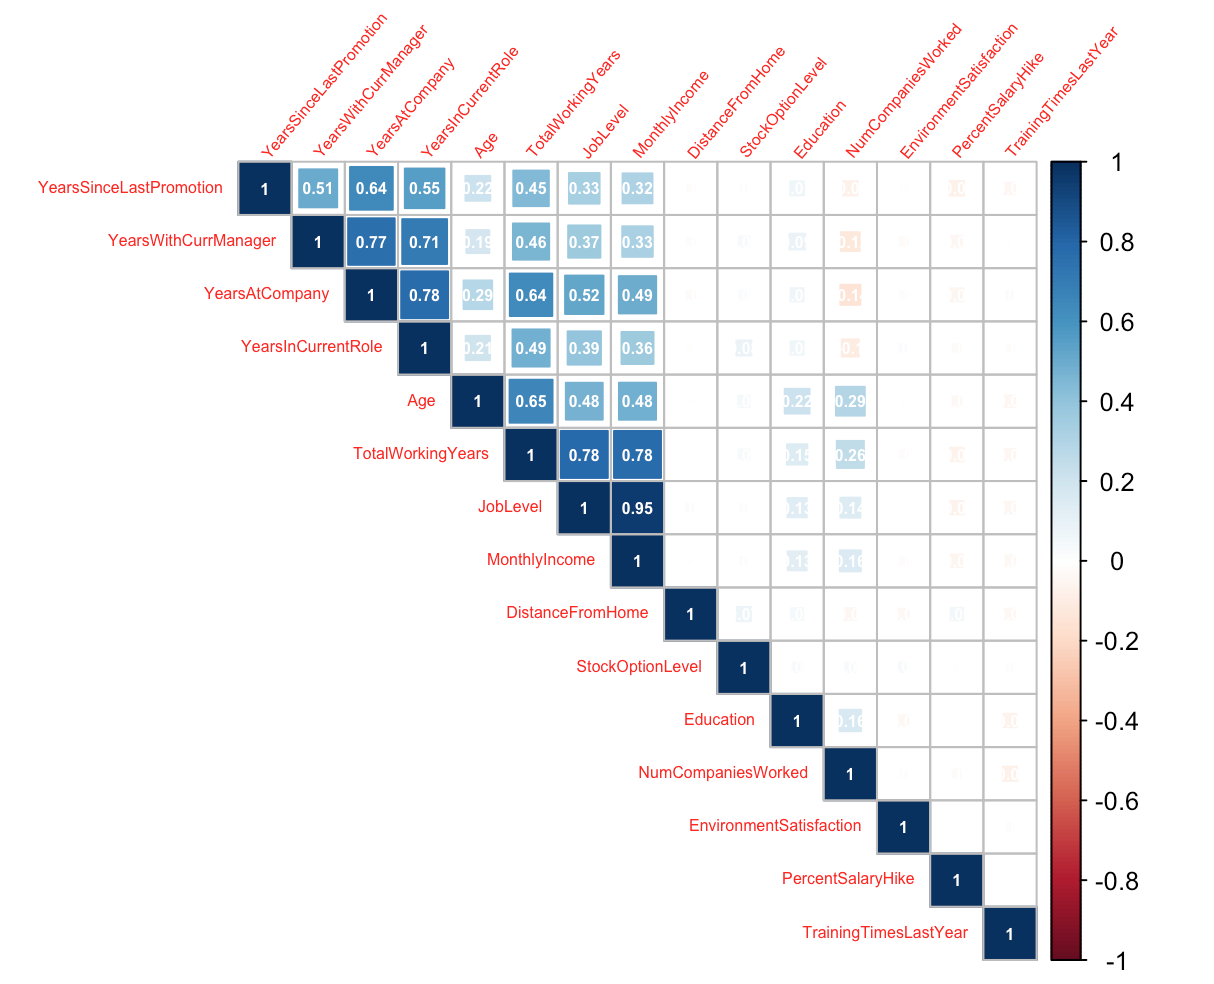
\includegraphics[scale=0.40]{PIC8}
\end{figure}


\end{frame}


%%%%%%%


%%%%%%%%%
\begin{frame}
\begin{center}
\textbf{\color{blue}\Large{Automated EDA - Monthly Income}}
\end{center}\medskip
\begin{figure}
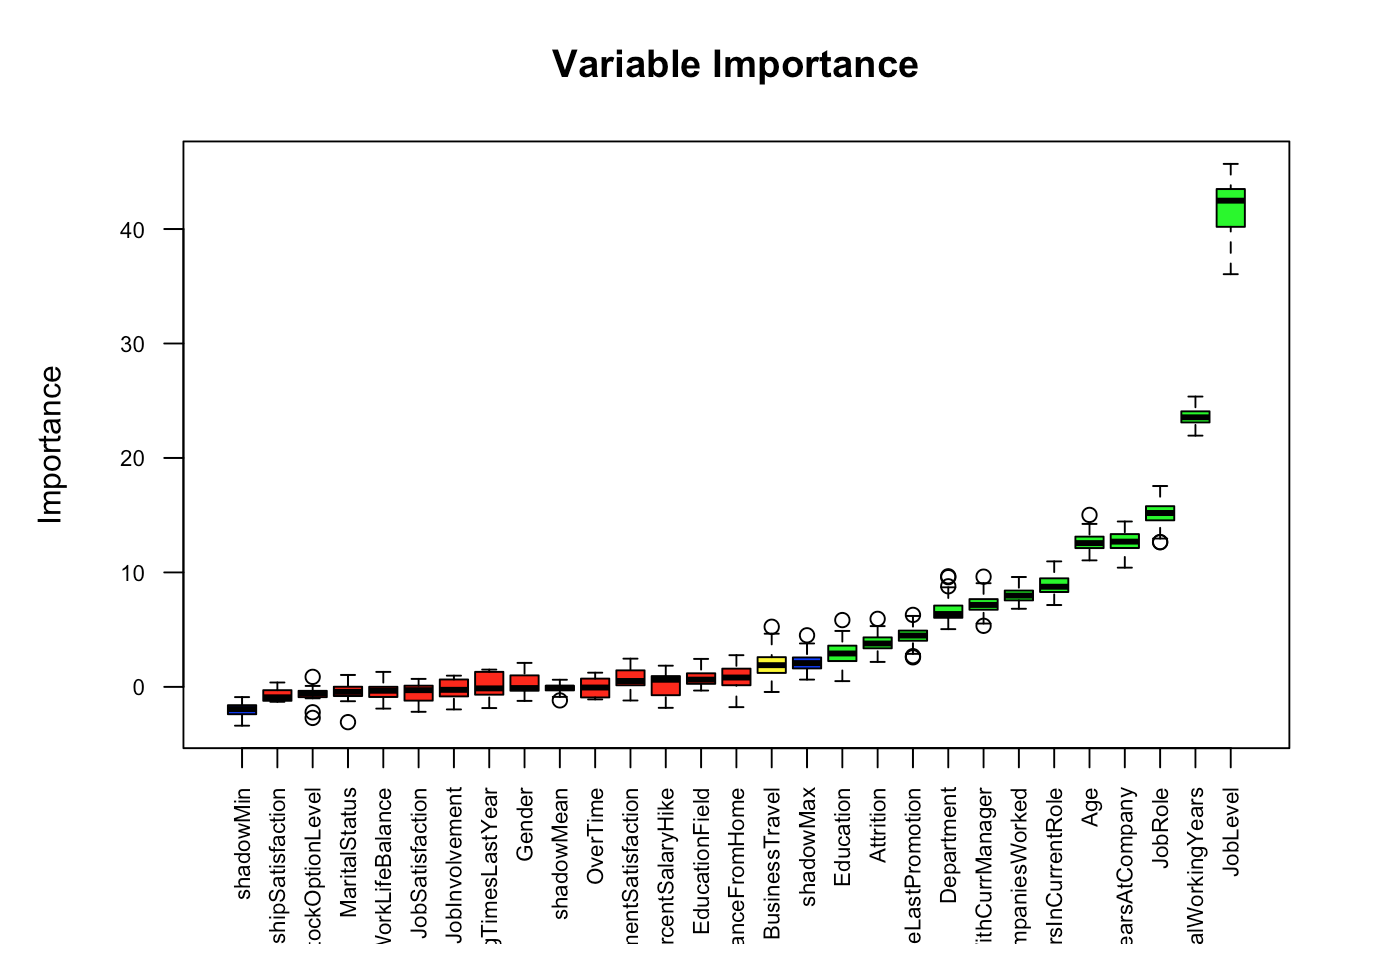
\includegraphics[scale=0.40]{PIC9}
\end{figure}


\end{frame}


%%%%%%%

%%%%%%%%%
\begin{frame}
\begin{center}
\textbf{\color{blue}\Large{Automated EDA - Attrition}}
\end{center}\medskip
\begin{figure}
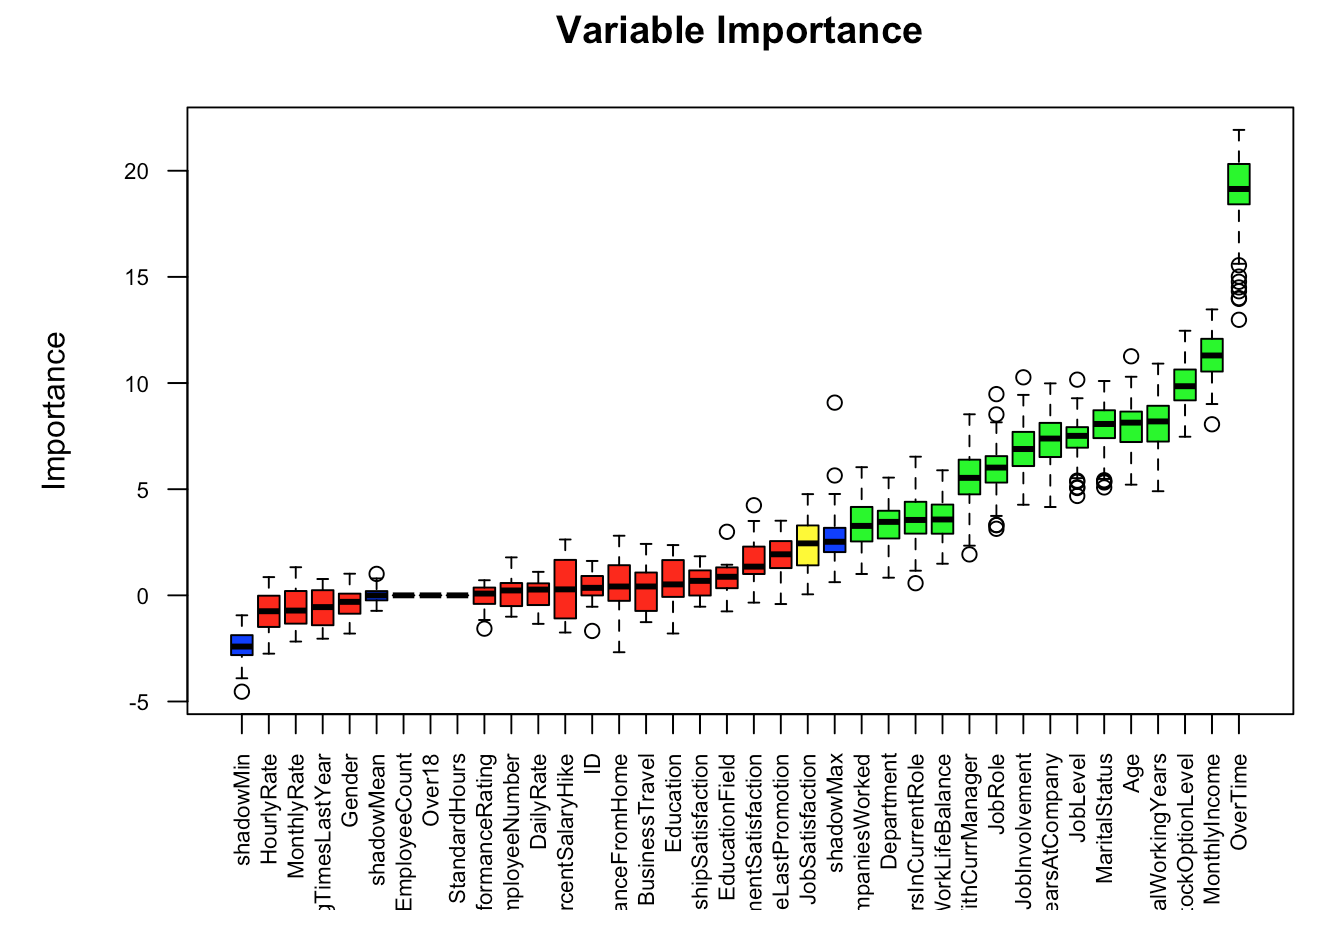
\includegraphics[scale=0.40]{PIC10}
\end{figure}


\end{frame}


%%%%%%%


%%%%%%%%%
\begin{frame}
\begin{center}
\textbf{\color{blue}\Large{Automated EDA - Attrition}}
\end{center}\medskip
\begin{figure}
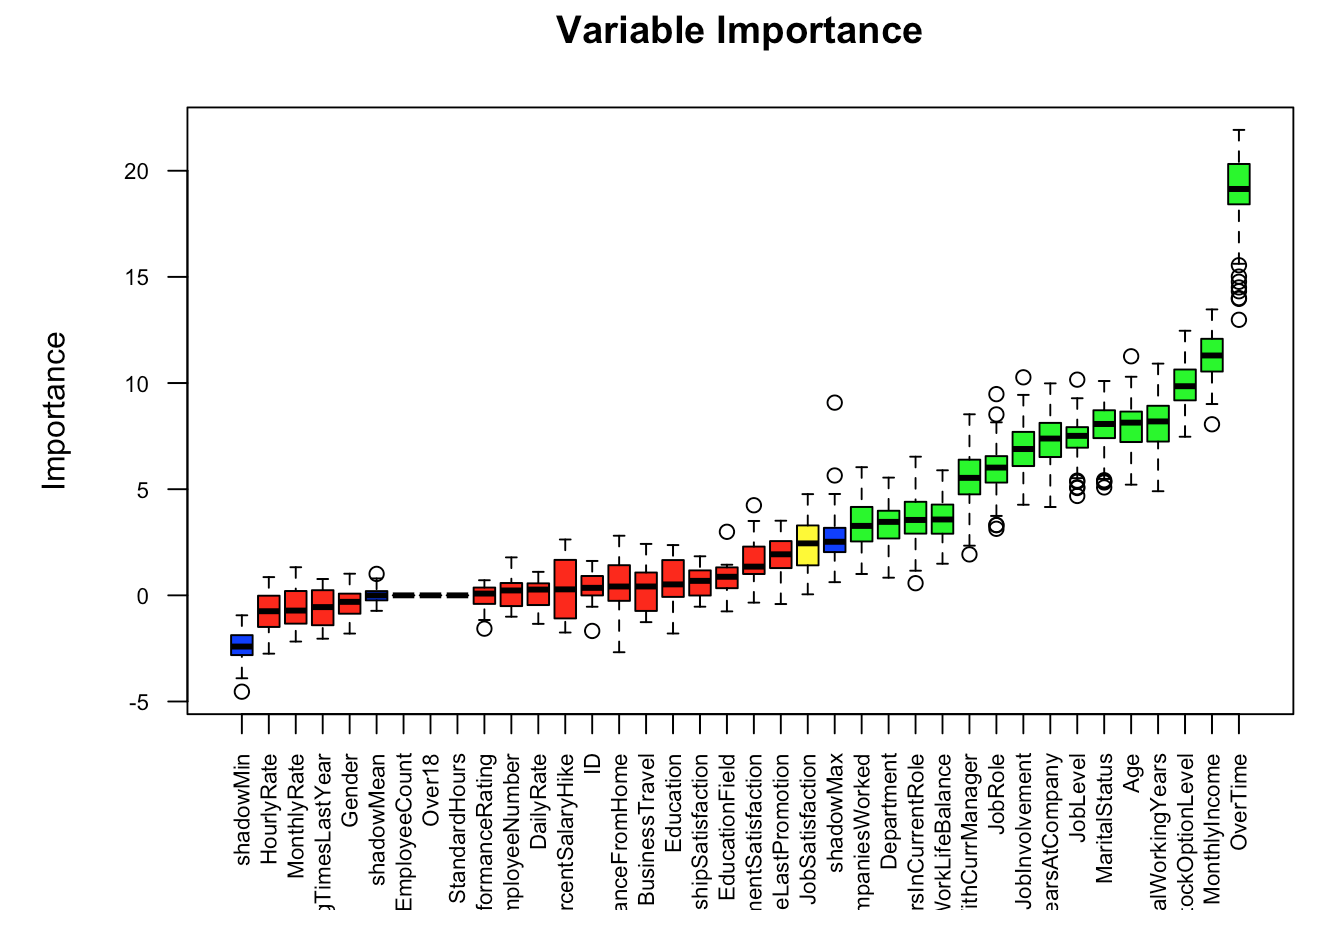
\includegraphics[scale=0.40]{PIC10}
\end{figure}


\end{frame}


%%%%%%%

%%%%%%%%%
\begin{frame}
\begin{center}
\textbf{\color{blue}\Large{Multiple Linear Regression and Validation for Salary}}
\end{center}
\begin{itemize}
\item<1-> Build a model by using multiple linear regression on Monthly Income related to 14 important variables: Age, Attrition, BusinessTravel, Department, Education, JobLevel, JobRole, NumCompaniesWorked, TotalWorkingYears, YearsAtCompany, YearsInCurrentRole, YearsSinceLastPromotion, YearsWithCurrManager.
\item<1 -> RMSE is around 1031.816 USD.
\item<1-> Validation for Salary.
\end{itemize}

\end{frame}


%%%%%


%%%%%%%%%
\begin{frame}
\begin{center}
\textbf{\color{blue}\Large{Naive Bayes classifiers  and Validation for Attrition}}
\end{center}
\begin{itemize}
\item<1-> Build a model by using Navie Bayes classifiers  on Attrition related to 17 important variables: Age, Department, EnvironmentSatisfaction, JobInvolvement, JobLevel, JobRole, JobSatisfaction, MaritalStatus, MonthlyIncome, NumCompaniesWorked, OverTime, StockOptionLevel, TotalWorkingYears, WorkLifeBalance, YearsAtCompany, YearsInCurrentRole, YearsWithCurrManager.
\end{itemize}
\begin{figure}
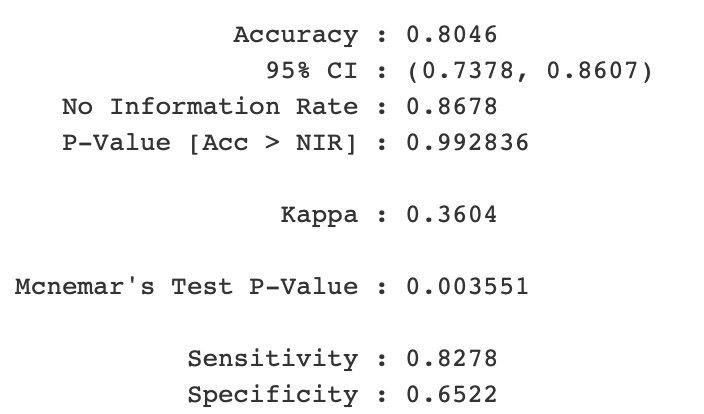
\includegraphics[scale=0.3]{PIC11}
\end{figure}
\begin{itemize}
\item<1-> Validation for Attrition
\end{itemize}
\end{frame}



\begin{frame}
\begin{center}
\textbf{\color{blue}\Large{Shiny App}}
\end{center}
\begin{itemize}
\item<1-> https://hnguye01.shinyapps.io/DDSAnalyticsApp/
\end{itemize}
\begin{figure}
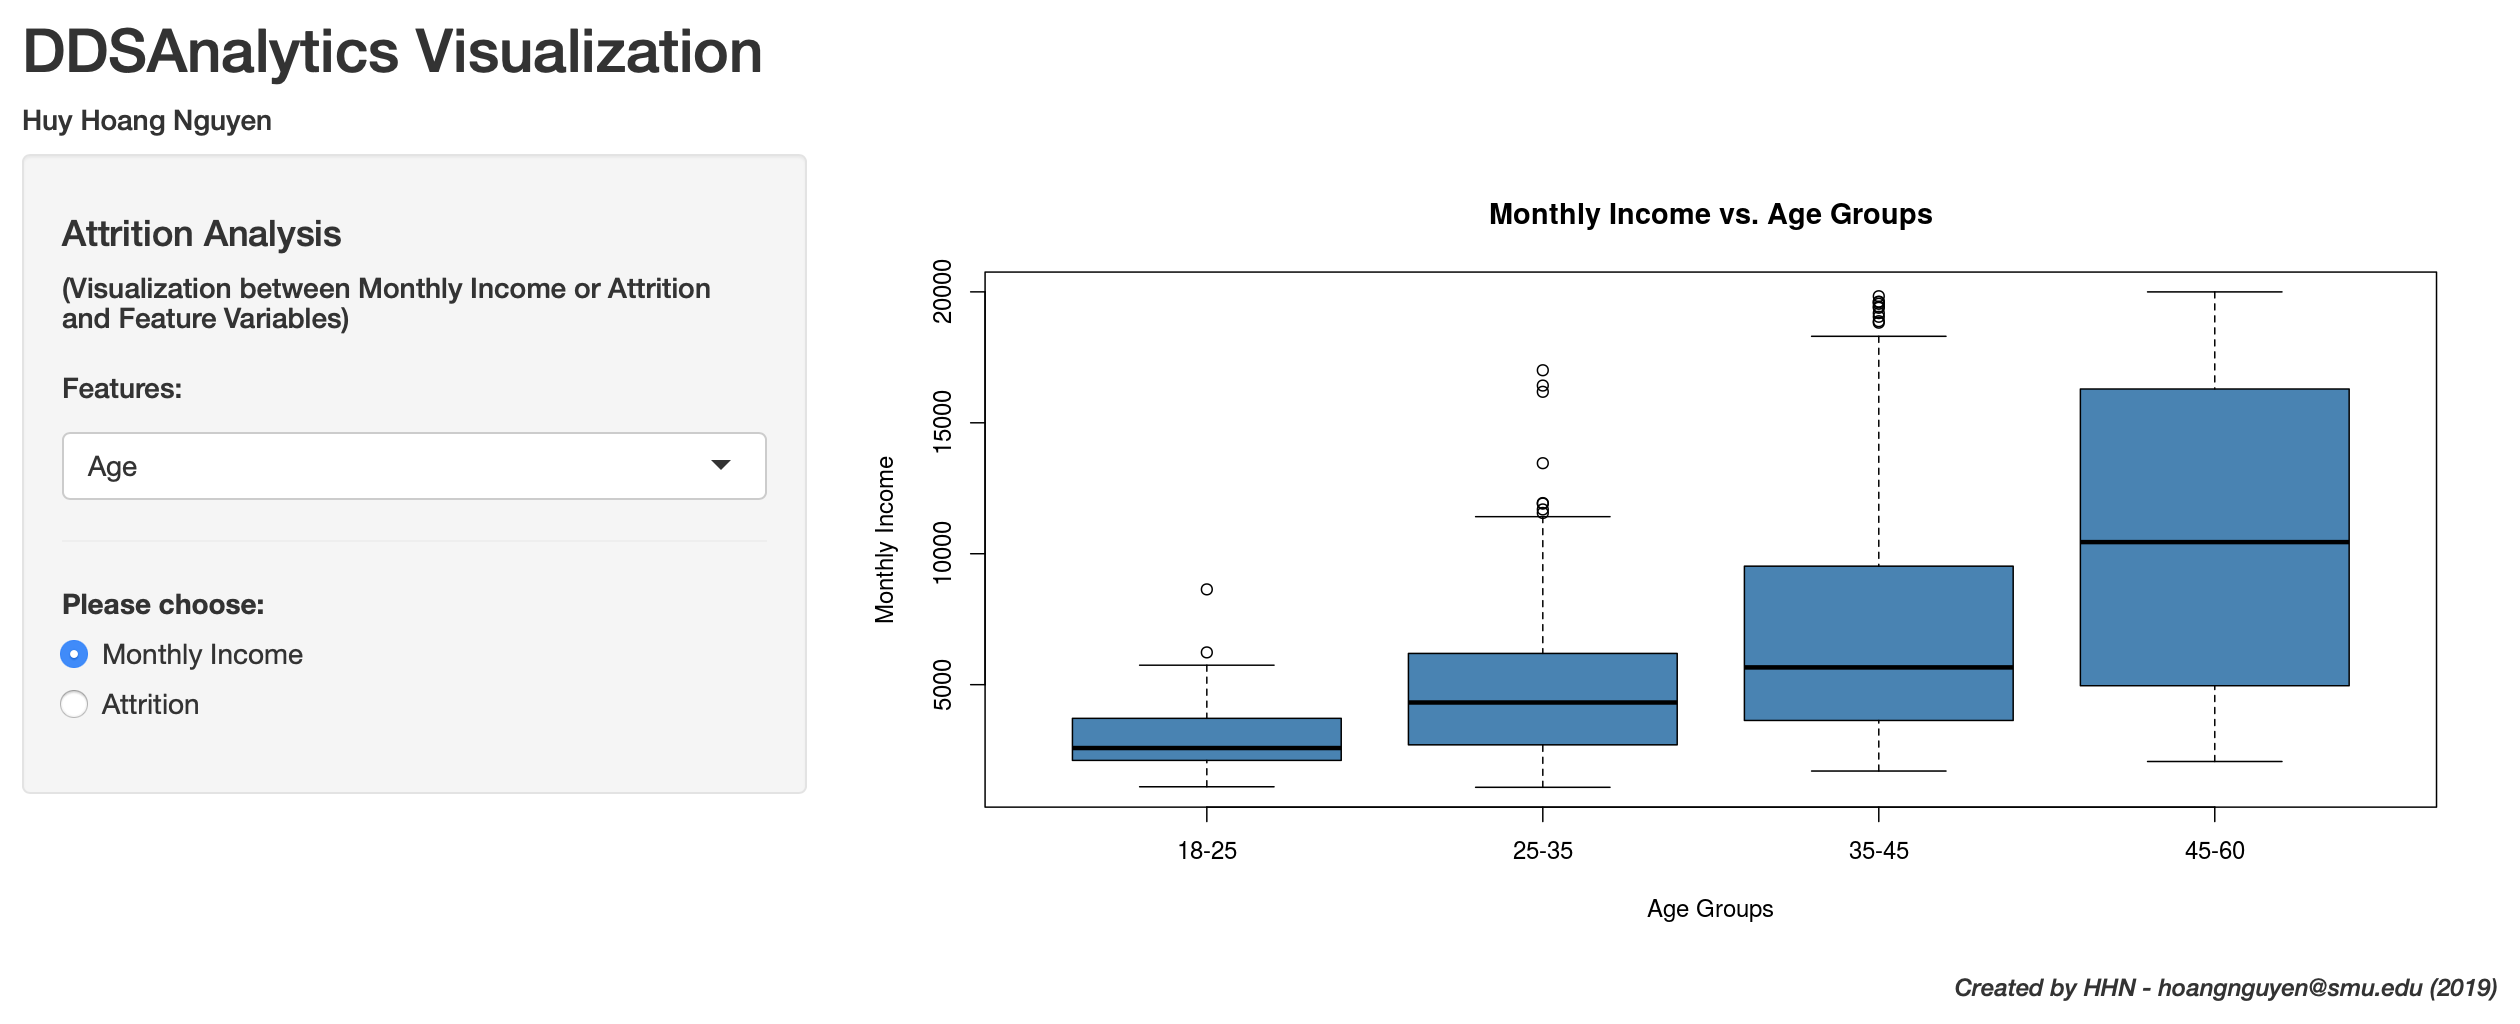
\includegraphics[scale=0.25]{PIC12}
\end{figure}
\end{frame}

%%%%%





\begin{frame}
\begin{center}
\textbf{\color{blue}\Large{Conclusion}}
\end{center}
\begin{itemize}
\item<1-> EDA to get information about important variables to build models  
\item<2-> Sales Representatives with highest rate and Manufacturing and Research Directors with the lowest rates in Attrition
\item<3-> Github link: https://github.com/hnguye01/6306two
\end{itemize}
\end{frame}


%%%%%%%

\begin{frame}

\begin{center}

\textbf{\color{red}Thank you for your attention}
\bigskip



\end{center}

\end{frame}

\end{document}









